\chapter{Results}
\label{cha:Results}
In this section, we will give some examples of generated reports obtained by passing a full program as input to the type extractor. The program analysis is not supposed to be fast. The overhead of a Lua call for each hook is high enough to leverage time performance. In this section we will present some reports generated by the extractor when analysing simple Lua programs and also Lua benchmark programs.

\section*{Basic}
A basic result of the extractor is represented by the Image~\ref{fig:basic1}. The output generated is related to the execution of Code~\ref{basic1}. Image~\ref{fig:basic2} shows the output for Code~\ref{basic2}. In this example, regardless of the input type, because the result generated by \textit{type} is always an string.
\lstinputlisting[label=basic1,title={Basic example 1},caption={Basic example 1}, language={[5.0]Lua}]{codes/basic_1.lua}
\lstinputlisting[label=basic2,title={Basic example 2},caption={Basic example 2}, language={[5.0]Lua}]{codes/basic_2.lua}
\begin{figure}
    \centering
    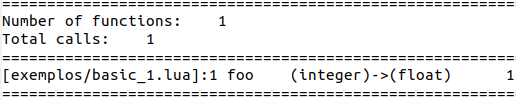
\includegraphics[width=0.65\textwidth]{pictures/basic1.png}
    \caption{Basic example 1}
    \label{fig:basic1}
\end{figure}
\begin{figure}
    \centering
    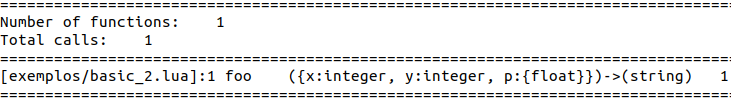
\includegraphics[width=0.85\textwidth]{pictures/basic2.png}
    \caption{Basic example 2}
    \label{fig:basic2}
\end{figure}
Another useful example is shown by the output of Code~\ref{basic3} and its output in Image~\ref{fig:basic3}. Instead of analysing transfered values only in the return event, the extractor analyses the parameter type in a call event, before any other assignment is made, preserving the type of the variables before the function's execution.
\lstinputlisting[label=basic3,title={Basic example 3},caption={Basic example 3}, language={[5.0]Lua}]{codes/basic_3.lua}
\begin{figure}
    \centering
    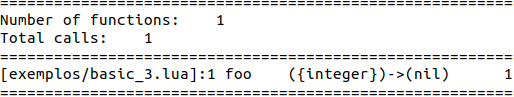
\includegraphics[width=0.85\textwidth]{pictures/basic3.png}
    \caption{Basic example 3}
    \label{fig:basic3}
\end{figure}
Image~\ref{fig:basic4} exeplifies a union of function types, generated by the execution of Code~\ref{basic4}. An union between an array of integer and a boolean type results in a dynamic type.
\lstinputlisting[label=basic4,title={Basic example 4},caption={Basic example 4}, language={[5.0]Lua}]{codes/basic_4.lua}
\begin{figure}
    \centering
    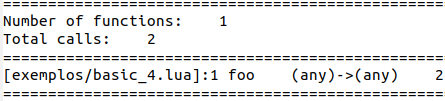
\includegraphics[width=0.85\textwidth]{pictures/basic4.png}
    \caption{Basic example 4}
    \label{fig:basic4}
\end{figure}
Finally, Image~\ref{fig:basic5} shows the handling of proper tail calls in action. Code~\ref{basic5} has two functions, where the last statement of \textit{foo} is a call to \textit{boo}, when the return event of this function is triggered, the return type of the calling function is updated correctly.
\clearpage
\lstinputlisting[label=basic5,title={Basic example 5},caption={Basic example 5}, language={[5.0]Lua}]{codes/basic_5.lua}
\begin{figure}
    \centering
    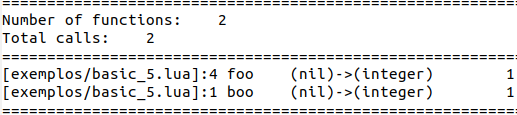
\includegraphics[width=0.85\textwidth]{pictures/basic5.png}
    \caption{Basic example 5}
    \label{fig:basic5}
\end{figure}









% \lstinputlisting[label=mean2,title={Mean Filter},caption={Mean Filter},language=R]{codes/mean.R}